% Created 2025-01-12 Sun 18:34
% Intended LaTeX compiler: pdflatex
\documentclass[11pt]{article}
\usepackage[utf8]{inputenc}
\usepackage[T1]{fontenc}
\usepackage{graphicx}
\usepackage{longtable}
\usepackage{wrapfig}
\usepackage{rotating}
\usepackage[normalem]{ulem}
\usepackage{amsmath}
\usepackage{amssymb}
\usepackage{capt-of}
\usepackage{hyperref}
\usepackage[polish]{babel}
\usepackage[T1]{fontenc}
\usepackage[utf8]{inputenc}
\selectlanguage{polish}
\usepackage{caption}
\usepackage{booktabs}
\captionsetup{labelfont=bf}
\usepackage{float}
\usepackage{svg}
\usepackage[a4paper, total={6.5in, 10in}]{geometry}
\author{Piotr Karamon}
\date{07.01.2025.}
\title{Laboratorium 10 cz. 1 - Teoria śladów}
\hypersetup{
 pdfauthor={Piotr Karamon},
 pdftitle={Laboratorium 10 cz. 1 - Teoria śladów},
 pdfkeywords={},
 pdfsubject={},
 pdfcreator={Emacs 29.2 (Org mode 9.7.11)}, 
 pdflang={Polish}}
\begin{document}

\maketitle
\section*{Treści zadań}
\label{sec:orge725ef2}
\subsection*{Zadanie 1}
\label{sec:org79dcfef}
Rozważmy zbiór zmiennych (''bazę danych'') \(x\), \(y\), \(z\)
i następujący zbiór akcji (''transakcji'') modyfikujących wartości tych zmiennych:

\begin{itemize}
\item (a) \(x := x + y\)
\item (b) \(y := y + 2z\)
\item (c) \(x := 3x + z\)
\item (d) \(z := y - z\)
\end{itemize}

Akcje możemy wykonywać współbieżnie z następującym zastrzeżeniem: akcja zmieniająca wartość zmiennej nie może być wykonana współbieżnie z akcją odczytującą lub modyfikującą stan tej samej zmiennej. W języku teorii śladów: dwie akcje są zależne jeśli obie operują na tej samej zmiennej, a przynajmniej jedna z nich modyfikuje wartość tej zmiennej.
\subsubsection*{Zadanie 1a}
\label{sec:org95b23ea}
W alfabecie \(A = \{a, b, c, d\}\) określ relacje zależności i niezależności.
\subsubsection*{Zadanie 1b}
\label{sec:org4a9932a}
Wyznacz ślad wyznaczony przez słowo \(w = baadcb\) względem powyższej relacji niezależności.
\subsubsection*{Zadanie 1c}
\label{sec:orgc7290c6}
Wyznacz postać normalną Foaty śladu \([w]\), można skorzystać z algorytmu z pracy
\emph{Volker Diekert, Yves Metivier: Partial Commutation and Traces, str. 11.}
\subsubsection*{Zadanie 1d}
\label{sec:orgdeca710}
Narysuj graf zależności Diekerta (w postaci zminimalizowanej - bez krawędzi "przechodnich") dla słowa \(w\).
\subsection*{Zadanie 2}
\label{sec:org870d3c3}
Dany jest zbiór akcji:

\begin{itemize}
\item (a) \(x \leftarrow y + z\)
\item (b) \(y \leftarrow x + w +y\)
\item (c) \(x \leftarrow x + y + v\)
\item (d) \(w \leftarrow v + z\)
\item (e) \(v \leftarrow x + v + w\)
\item (f) \(z \leftarrow y + z+ v\)
\end{itemize}
\subsubsection*{Zadanie 2a}
\label{sec:org80aa92a}
W alfabecie \(A = \{ a, b, c, d, e, f \}\) określ relacje zależności i niezależności.
\subsubsection*{Zadanie 2b}
\label{sec:orgbda5a46}
Wyznacz postać normalną Foaty śladu \([u]\), gdzie \(u = acdcfbbe\).
\subsubsection*{Zadanie 2c}
\label{sec:org830e540}
Narysuj graf zależności Diekerta (w postaci zminimalizowanej - bez krawedzi "przechodnich") dla słowa \(u\).
\section*{Zadanie 1}
\label{sec:orgfefbdec}
Mamy następujące akcje

\begin{itemize}
\item (a) \(x := x + y\)
\item (b) \(y := y + 2z\)
\item (c) \(x := 3x + z\)
\item (d) \(z := y - z\)
\end{itemize}

Relacja zależność \(D\), jest relacją symetryczną i refleksywną, zatem:
\begin{align*}
D &= \text{sym} \{ (a,b), (a,c), (b,d), (c,d) \} \cup I_A = \\
&= \{(a,a), (b,b), (c, c), (d,d), (a, b), (b, a), (a, c), (c,a), (b, d), (d, b), (c, d), (d, c)\}
\end{align*}

Relacja niezależności to \(I = A^2 - D\), zatem:

\begin{align*}
I = \{(a, d), (b, c), (c, b), (d, a) \}
\end{align*}

Aby wyznaczyć ślad dla słowa \(w = baadcb\) korzystamy ze zbioru \(I\) i zamieniamy
kolejność sąsiednich operacji, jeżeli są one niezależne.

$$[baadcb]_I = \{baadcb, badacb, baadbc, bdaacb, badabc, baadbc   \}$$

Aby wyznaczyć postać normalną Foaty dla śladu \([w]\) wykorzystujemy podany algorytm.

$$[w] = (b)(ad)(a)(bc)$$

Aby stworzyć graf Diekerta dla słowa \(baadcb\) najpierw tworzymy graf, w którym krawędź występuje jeżeli dwie akcje są zależne, ale jest to krawędź skierowana.

\begin{figure}[H]
\centering
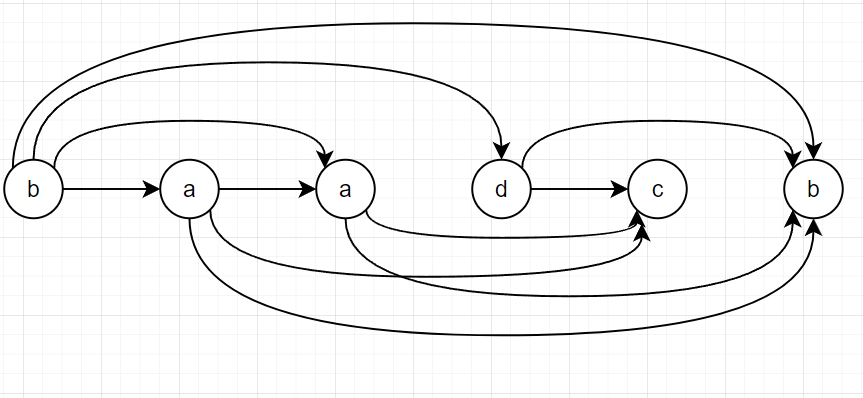
\includegraphics[width=.9\linewidth]{./graph1_1.png}
\caption{Graf Diekerta wraz z krawędziami przechodnimi dla słowa \(w\).}
\end{figure}

Następnie usuwamy krawędzie przechodnie, w rezultacie dostajemy graf:

\begin{figure}[H]
\centering
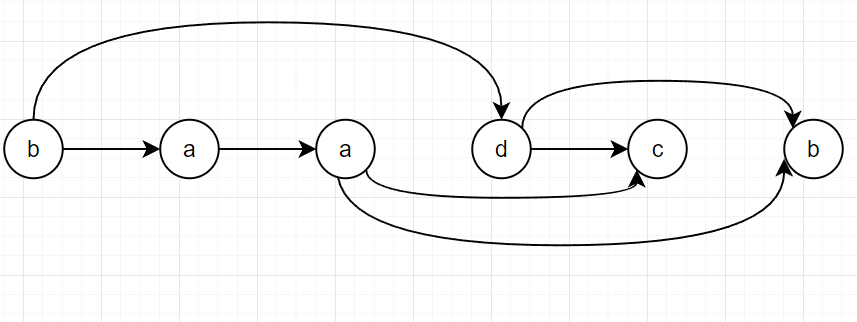
\includegraphics[width=.9\linewidth]{./graph1_2.png}
\caption{Graf Diekerta w postaci zminimalizowanej dla słowa \(w\).}
\end{figure}

Dla lepszej czytelności możemy trochę poprzemieszczać elementy grafu. Do wygenerowania grafu użyjemy PlantUML.

\begin{figure}[H]
\centering
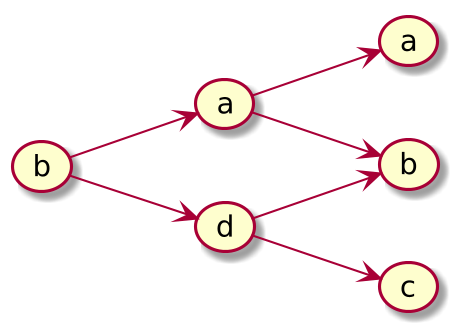
\includegraphics[width=0.6\linewidth]{graph1.png}
\caption{\label{}Graf Diekerta w postaci zminimalizowanej dla słowa \(w\).}
\end{figure}
\section*{Zadanie 2}
\label{sec:orgd442adc}
Dany jest zbior akcji:
\begin{itemize}
\item (a) \(x \leftarrow y + z\)
\item (b) \(y \leftarrow x + w +y\)
\item (c) \(x \leftarrow x + y + v\)
\item (d) \(w \leftarrow v + z\)
\item (e) \(v \leftarrow x + v + w\)
\item (f) \(z \leftarrow y + z+ v\)
\end{itemize}

Relacja zależności:

$$ D = I_A \cup \text{sym}\{(a,b), (a, c), (a, e), (a,f), (b, c), (b, d), (b,f), (c,e), (d, e), (d, f), (e, f)\}$$

Relacja niezależności:

$$ I = \text{sym} \{(a, d), (b, e), (c, d), (c, f)  \}$$

Postać normalna Foata śladu \([u]\), gdzie \(u=acdcfbbe\).
Wykorzystujemy podany algorytm i otrzymujemy:
$$[u] = (ad)(cf)(c)(be)(b)$$


\begin{figure}[H]
\centering
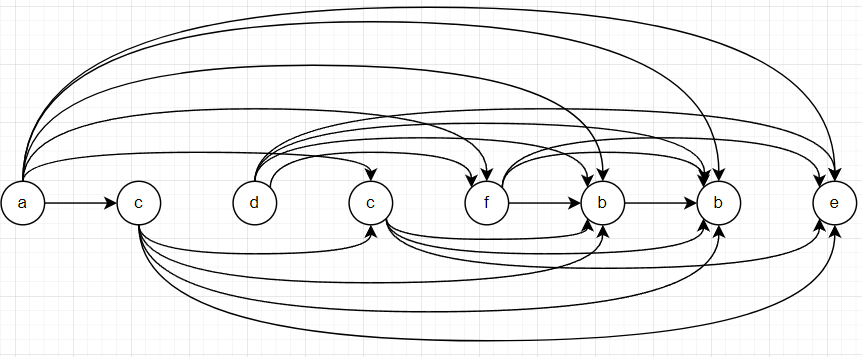
\includegraphics[width=.9\linewidth]{./graph2_1.png}
\caption{Graf Diekerta wraz z krawędziami przechodnimi dla słowa \(u\).}
\end{figure}


\begin{figure}[H]
\centering
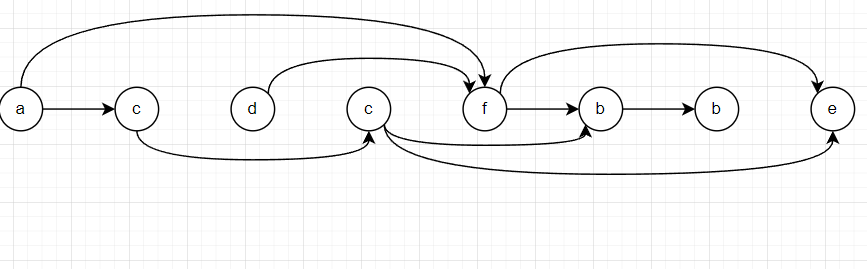
\includegraphics[width=.9\linewidth]{./graph2_2.png}
\caption{Graf Diekerta w postaci zminimalizowanej dla słowa \(u\).}
\end{figure}


\begin{figure}[H]
\centering
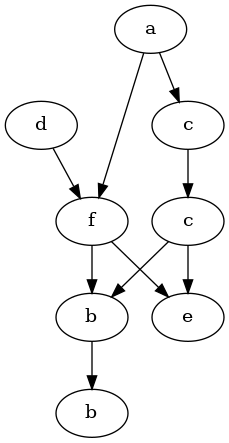
\includegraphics[width=0.4\linewidth]{graph2.png}
\caption{\label{}Graf Diekerta w postaci zminimalizowanej dla słowa \(u\).}
\end{figure}
\section*{Bibliografia}
\label{sec:org7b0c724}
\begin{itemize}
\item \href{https://www.researchgate.net/publication/280851316\_Partial\_Commutation\_and\_Traces}{Volker Diekert, Yves Metivier : Partial Commutation and Traces}
\item \href{https://plantuml.com/guide}{PlantUML Language Reference}
\end{itemize}
\end{document}
